\section{Laboratory work implementation}

\subsection{Tasks and Points}

\begin{itemize}
	\item for Basic Level (grade 5 || 6):
				\begin{itemize}
					\item Simple site with 3 static pages
				\end{itemize}
	\item for Normal Level (grade 7 || 8):
			\begin{itemize}
				\item Your site must keep all site data in a database.
			\end{itemize}
	\item for Advanced Level (grade 9 || 10):
		\begin{itemize}
			\item Your site must contain AJAX Requests.
			\item Your controllers must implement XHR or JSON responses. Some Data are dynamically loaded to the page.
		\end{itemize}
\end{itemize}


\subsection{Analiza lucrarii de laborator}

Pentru realizarea unui site in primul rind avem nevoie de un server, pentru aceasta mi-am creeat un sub-domen pe site-ul byethost.com, unde prin ftp m-am conectat pentru upload-ul filerurilor.
Am initializat 2 file-uri html si unul php.
In prima pagina am folosit majoritatea resurselor foundation.zurb care includ apelarea scripturilor java-script si jquerry pentru implementarea full-responsive la redimensionarea ferestrei. Am stilizat prin file-ul .css pagina html. Am folosit hover pentru disparitia unui element prin opacity 0, am implementat un Top-Menu responsive cu lincurile la toate paginile si drop-down list . El ne ajuta sa navigam pe site
\begin{center}

\includegraphics[width=0.7\linewidth]{1}
\end{center}
Si versiunea mobila:
\begin{center}

\includegraphics[width=0.7\linewidth]{2}
\end{center}
Dupa care am introdus text prin <p> si <h1> care este stilizat in css ca stil, culoare si pozitie
\begin{center}

\includegraphics[width=0.7\linewidth]{3}
\end{center}
Am introdus o imagine prin <img> pe full-width
\begin{center}

\includegraphics[width=0.7\linewidth]{4}
\end{center}
Am divizat urmatoarea zona in 2 pentru latimea ecranurilor calculatoarelor si cite un element unul sub altul in cazul deschiderii site-ului de pe mobil
Din resursele foundation am introdus un Orbit-slider (galerie foto)
\begin{center}
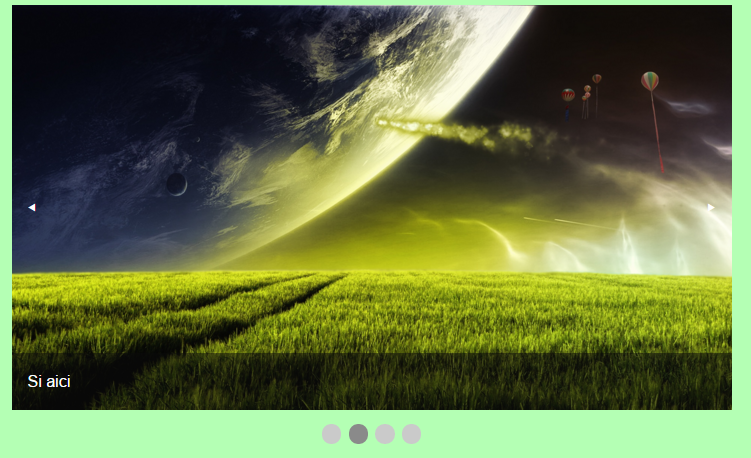
\includegraphics[width=0.7\linewidth]{5}
\end{center}
Prin javascript am introdus checkboxuri care la click afiseaza un text:
\begin{center}

\includegraphics[width=0.5\linewidth]{6}
\end{center}
Am introdus un buton:
\begin{center}

\includegraphics[width=0.7\linewidth]{7}
\end{center}
Care deschide un Reveal ce se afiseaza ca un dialog box si include text, imagine si 2 forms de text si un buton:
\begin{center}

\includegraphics[width=0.7\linewidth]{8}
\end{center}
Am folosit pozitia absoluta pentru a fixa un element ce se va misca dupa indeferent de scroll
\begin{center}

\includegraphics[width=0.4\linewidth]{9}
\end{center}
In pagina 3 am introdus iframe din youtube:
\begin{center}

\includegraphics[width=0.7\linewidth]{10}
\end{center}
Si un iframe la facebook:
\begin{center}

\includegraphics[width=0.7\linewidth]{11}
\end{center}
Dupa care, manual prin jquerry am reusit la tastarea pe zona de culoare rosie a elementului sa obtinem un expand lent ce ne afiseaza textul de pe fon galben:
\begin{center}
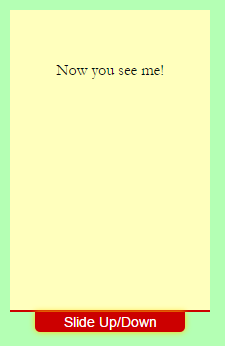
\includegraphics[width=0.3\linewidth]{12}
\end{center}
Pe pagina 2 am introdus reusit sa implementez afisarea partiala a unei baza de date, care fara sa reincarce pagina afiseaza o anumita parte din content, pentru a creea o baza de date, am creeat-o in mySql 
\begin{center}

\includegraphics[width=0.7\linewidth]{../../../pentruSite/11}
\end{center}
Dupa care in phpMyAdmin am conectat-o

\begin{center}
\includegraphics[width=0.7\linewidth]{../../../pentruSite/13}
\end{center}
Astfel in acest menu importam o baza de date:
	
\begin{center}
\includegraphics[width=0.5\linewidth]{../../../pentruSite/15}
\end{center}

\begin{center}
\includegraphics[width=0.7\linewidth]{../../../pentruSite/16}
\end{center}
In file-ul php schimbind doar datele ce tin de logare

\begin{center}
\includegraphics[width=0.7\linewidth]{../../../pentruSite/17}
\end{center}
Aceasta pagina arata astfel:
\begin{center}
\includegraphics[width=0.7\linewidth]{13}
\end{center}

Am mai incercat sa conectez un php form pentru trimiterea mail-urilor:
\begin{center}
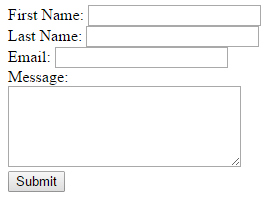
\includegraphics[width=0.7\linewidth]{14}
\end{center}
Care are nevoie la fel de schimbarea codului pentru emailul destinatiei.

\clearpage